\documentclass[a4paper,10pt]{article}
\usepackage[paper=a4paper, hmargin=1.5cm, bottom=1.5cm, top=3.5cm]{geometry}

\usepackage[utf8]{inputenc} %Codificacion de caracteres, para poder usar acentos, etc.
\usepackage[T1]{fontenc}
\usepackage[spanish]{babel}
\usepackage{xspace}
\usepackage{xargs} %Para crear funciones con muchos argumentos
\usepackage{ifthen}
\usepackage{aed2-tad,aed2-symb,aed2-itef,caratula} %Macros de Algo2
\usepackage{algorithm}% http://ctan.org/pkg/algorithms
\usepackage{algpseudocode} % Para algorritmia
%\usepackage{algorithmic} %paquete para hacer pseudocodigo

\usepackage{titlesec}%http://foro-c.com/blog/latex-formato-de-titulos-de-capitulos-secciones-etc/
\usepackage{graphicx} %Inlcuir imagenes.
\usepackage{setspace}
\usepackage{fancyhdr}
\usepackage[colorlinks=true, linkcolor=blue]{hyperref} %Links para el indice.
\usepackage{float} %Insercion de imagenes flotantes
\usepackage{ stmaryrd }

\usepackage{caption}
\usepackage{subcaption}

\newcommand{\moduloNombre}[1]{\textbf{#1}}

\let\NombreFuncion=\textsc
\let\TipoVariable=\texttt
\let\ModificadorArgumento=\textbf
\newcommand{\res}{$res$\xspace}
\newcommand{\tab}{\hspace*{7mm}}

\newcommandx{\TipoFuncion}[3]{%
  \NombreFuncion{#1}(#2) \ifx#3\empty\else $\to$ \res\,: \TipoVariable{#3}\fi% nombreFuncion(parametros) -> res:(Tipo)
}
\newcommand{\In}[2]{\ModificadorArgumento{in} \ensuremath{#1}\,: \TipoVariable{#2}\xspace}
\newcommand{\Out}[2]{\ModificadorArgumento{out} \ensuremath{#1}\,: \TipoVariable{#2}\xspace}
\newcommand{\Inout}[2]{\ModificadorArgumento{in/out} \ensuremath{#1}\,: \TipoVariable{#2}\xspace}
\newcommand{\Aplicar}[2]{\NombreFuncion{#1}(#2)}

\newlength{\IntFuncionLengthA}
\newlength{\IntFuncionLengthB}
\newlength{\IntFuncionLengthC}
%InterfazFuncion(nombre, argumentos, valor retorno, precondicion, postcondicion, complejidad, descripcion, aliasing)
\newcommandx{\InterfazFuncion}[9][4=true,6,7,8,9]{%
  \hangindent=\parindent
  \TipoFuncion{#1}{#2}{#3}\\%
  \textbf{Pre} $\equiv$ \{#4\}\\%
  \textbf{Post} $\equiv$ \{#5\}%
  \ifx#6\empty\else\\\textbf{Complejidad:} #6\fi%
  \ifx#7\empty\else\\\textbf{Descripcion:} #7\fi%
  \ifx#8\empty\else\\\textbf{Aliasing:} #8\fi%
  \ifx#9\empty\else\\\textbf{Requiere:} #9\fi%
}

\newenvironment{Algoritmos}{%
  \vspace*{2ex}%
  \noindent\textbf{}%
  \vspace*{2ex}%
}{}


\newcommand{\Titulo}[1]{
  \vspace*{1ex}\par\noindent\textbf{\large #1}\par
}

\newcommand{\DRef}{\ensuremath{\rightarrow}}

\newcommandx{\Algoritmo}[4]{%
	\noindent\TipoFuncion{#1}{#2}{#3}
	\begin{algorithmic}[1]
	#4
	\end{algorithmic}
}%

\newcommand{\nom}[1]{\NombreFuncion{#1}}

\newcommand{\comp}[1]{\hfill \ensuremath{O(#1)}}
\newcommand{\compTot}[1]{\hfill \textbf{Complejidad Total: }\ensuremath{O(#1)}}

\sloppy

\hypersetup{%
 % Para que el PDF se abra a pagina completa.
 pdfstartview= {FitH \hypercalcbp{\paperheight-\topmargin-1in-\headheight}},
 pdfauthor={C\'atedra de Algoritmos y Estructuras de Datos III - DC - UBA},
 pdfkeywords={},
 pdfsubject={}
}

\parskip=5pt % 10pt es el tamano de fuente

% Pongo en 0 la distancia extra entre itemes.
\let\olditemize\itemize
\def\itemize{\olditemize\itemsep=0pt}

% Acomodo fancyhdr.
\pagestyle{fancy}
\thispagestyle{fancy}
\addtolength{\headheight}{1pt}
\lhead{Algoritmos y Estructuras de Datos III}
\rhead{TP 3}
% \lhead{Algoritmos y Estructuras de Datos II}
% \rhead{$1^{\mathrm{do}}$ cuatrimestre de 2006}
%\cfoot{\thepage /\pageref{LastPage}}
%\renewcommand{\footrulewidth}{0.4pt}

\author{}
\date{01-07-2013}
\title{Trabajo}

\begin{document}
 
\materia{Algoritmos y Estructuras de Datos III}
\subtitulo{}
\titulo{Trabajo Pr\'actico 2}
\grupo{}

\integrante{Laura Muiño}{399/11}{mmuino@dc.uba.ar}
\integrante{Mart\'in Santos}{413/11}{martin.n.santos@gmail.com}
\integrante{Luis Toffoletti}{827/11}{luis.toffoletti@gmail.com	}
\integrante{Florencia Zanollo}{934/11}{florenciazanollo@hotmail.com}

\maketitle
\tableofcontents

\newpage

\section{Ejercicio 1}
\subsection{Descripción}
Se tienen n servidores interconectados mediante m enlaces. Los enlaces tienen un costo en función del tráfico que transmiten y todos los enlaces deben transmitir la misma información. El problema a resolver consiste en seleccionar aquellos enlaces que permitan distribuir la información a los n servidores con costo total mínimo.


Veamos un ejemplo; el siguiente grafo tiene como posible solución el subgrafo en rojo cuyo peso total es 38.

\begin{center}
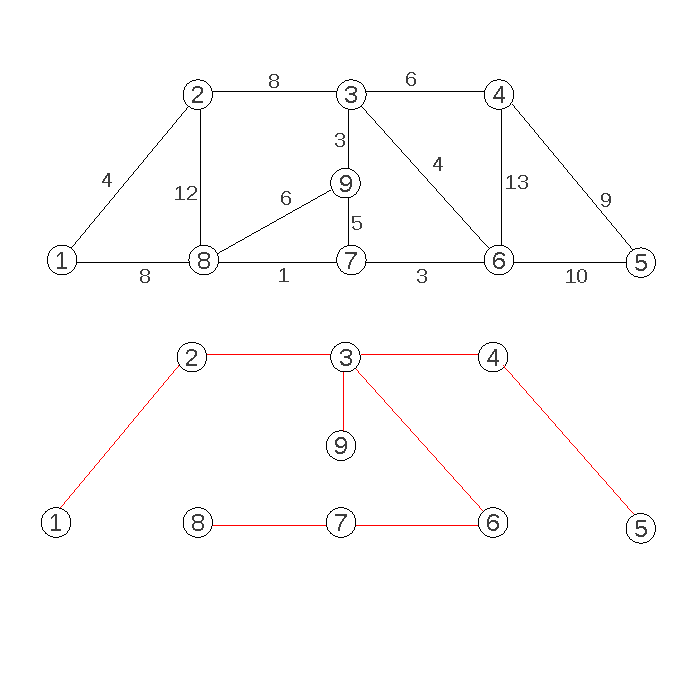
\includegraphics{ej2/1/Img1.pdf} 
\end{center}


\newpage
\subsection{Pseudocódigo:}

\begin{algorithm}
\caption{Impresiones ordenadas}\label{ej1}
\begin{algorithmic}[1]
\Procedure{Dividir trabajos}{$n, Costos$}\Comment{n= cant trabajos, Costos= costo de cada trabajo respecto a cada posible anterior}
	\State Inicializo una matriz dp, tamaño n*n
	
	\State dp[0][1]$\gets Costos(1,0)$ \Comment{en la posición (0,1) de la matriz guardo el valor de hacer el trabajo uno primero}
	
	\State $agregar\_a\_maquina2(1)$ \Comment{voy guardando los trabajos para saber al final cómo los dividí}
	
	\For{$j\gets 2, n$} \Comment{el trabajo 1 ya lo agregué}
		\For{$i\gets 0, j-1$}
			\If{$i=j-1$}
				\State $dp[i][j]\gets minimo(dp[i][k]\ +\ Costos(j,\ k),\ \forall\ 0\leq k\leq j-2) $
				\State $agregar\_a\_maquina2(j)$
				
			\Else
				\State $dp[i][j]\gets (dp[i][j-1]\ +\ Costos(j,\ j-1))$
				\State $agregar\_a\_maquina2(j)$
			\EndIf
		\EndFor
	\EndFor
	
	\State \textbf{return} $minimo(dp[i][n], \forall\ 0\leq i\leq n-1)$ 
	\State \Comment{retorno el mínimo de la última columna, además de la combinación para lograr ese mínimo}
\EndProcedure
\end{algorithmic}
\end{algorithm}

\textit{Nota:} Cuando escribo $agregar\_a\_maquina2(j)$ me refiero a agregar j a una lista que depende de la posición de la matriz dp (i.e. hay una para cada posición).\\
\subsection{Complejidad}

%The running time of Prim’s algorithm depends on how we implement the min-
%priority queue Q. If we implement Q as a binary min-heap (see Chapter 6), we
%can use the B UILD -M IN -H EAP procedure to perform lines 1–5 in O.V / time. The
%body of the while loop executes jV j times, and since each E XTRACT-M IN opera-
%tion takes O.lg V / time, the total time for all calls to E XTRACT-M IN is O.V lg V /.
%The for loop in lines 8–11 executes O.E/ times altogether, since the sum of the
%lengths of all adjacency lists is 2 jEj. Within the for loop, we can implement the
%test for membership in Q in line 9 in constant time by keeping a bit for each vertex
%that tells whether or not it is in Q, and updating the bit when the vertex is removed
%5from Q. The assignment in line 11 involves an implicit D ECREASE -K EY opera-
%tion on the min-heap, which a binary min-heap supports in O.lg V / time. Thus,
%the total time for Prim’s algorithm is O.V lg V C E lg V / D O.E lg V /, which is
%asymptotically the same as for our implementation of Kruskal’s algorithm.

La complejidad de Prim Modificado dependerá de la estructura utilizada para ir eligiendo aristas. El cuerpo del while se ejecuta C veces. El obtener mínimo dentro del while se ejecutará O(R) veces en total en donde cada operación de push, pop cuesta log(R) lo que equivale a O(log $(F+C)^2$) ya que $(F+C)^2$ es la mayor cantidad de aristas posibles. Como F es menor que C (enunciado), log($(C+F)^2$) $\subset$ log($C^2$). Por lo tanto la complejidad equivale a O(2 log C) $\subset$ O(log C). El for que se encarga de pushear las aristas adyacentes a la cola de prioridad también se ejecutará un total de R veces y la operación de push cuesta log(R) $\subset$ O(log C). Por lo tanto la complejidad total será de O(R*log(C)+R*log(C)) $\subset$ O(R*log(C)) como pedía el enunciado.

\subsection{Demostración}

Diremos que un conjunto de aristas factible es $prometedor$ si se puede extender para producir no sólo una solución, sino una solución óptima para nuestro problema. Si un conjunto de aristas prometedor ya es solución entonces esta solución debe ser óptima.

La demostración de la correctitud de algoritmo es por inducción sobre el número de aristas que hay en el conjunto T. Demostraremos que si T es prometedor en alguna fase del algoritmo, entonces sigue siendo prometedor al añandir una arista adicional. Cuando se detiene el agoritmo (T tiene C cantidad de aristas), T da una solución prometedora al problema y por lo tanto óptima.

Caso base: el conjunto vacío T es prometedor
Paso inductivo: supongamos que T es prometedor justo antes de que el algoritmo añada una nueva arista $e$ al conjunto T. T es un conjunto de aristas prometedor por hipótesis inductiva y $e$ es por definición una de las aristas más cortas que salen de B. Podemos asegurar que existe un $e$ que cumpla dichos requisitos ya que el enunciado asegura que todos los clientes pueden ser provistos por al menos una fábrica. Por lo tanto T $\cup$ $e$ también es prometedor.

Como el conjunto T es prometedor en todas las fases del algoritmo también lo será cuando finalice ya que ofrece una solción óptima del problema.

\subsection{Casos de Prueba}

Vamos a presentar 5 instancias distintas del problema mediante gr´aficos, y la soluci´on que nos devuelve la implementaci´on, de manera de hacer una comprobaci´on visual del funcionamiento.

\begin{center}
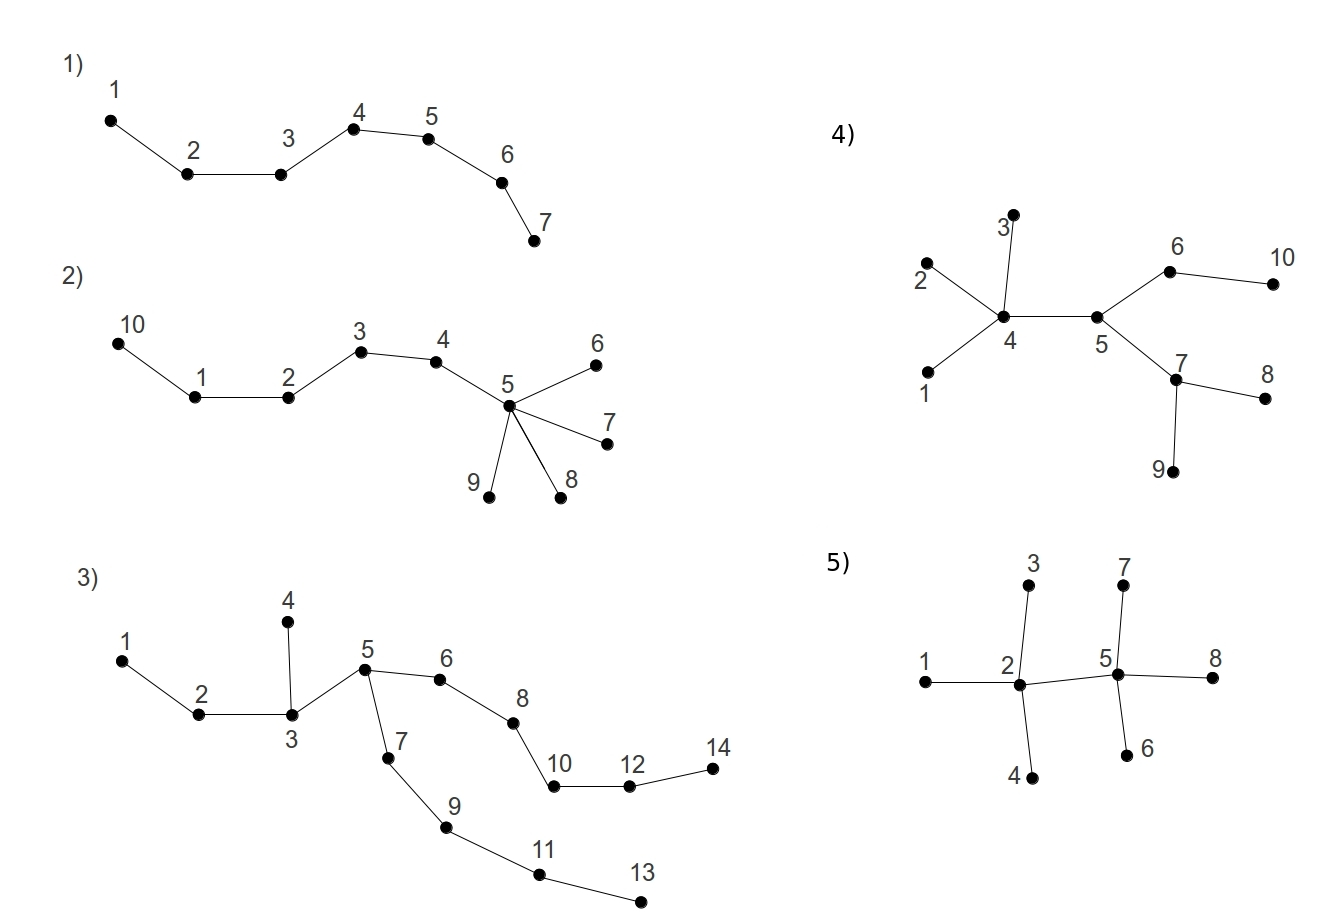
\includegraphics[scale=0.5]{ej2/2/graficos/imagen05.jpg} 
\end{center}

\begin{center}
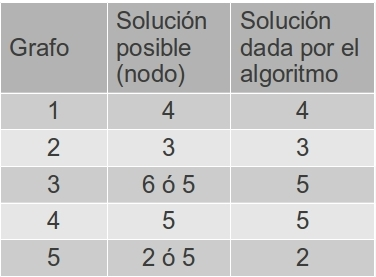
\includegraphics[scale=0.5]{ej2/2/graficos/imagen06.jpg} 
\end{center}
\newpage
\subsection{Experimentación:}

Se realizaron experimentos con instancias aleatorias, generadas utilizando la función rand()\footnote{http://www.cplusplus.com/reference/cstdlib/rand/}  perteneciente a la Standard Library.

Los experimentos se ejecutaron varias veces, para instancias diferentes, contando la cantidad de ciclos que conlleva resolver el problema y luego se promediaron los datos obtenidos.

\begin{center}
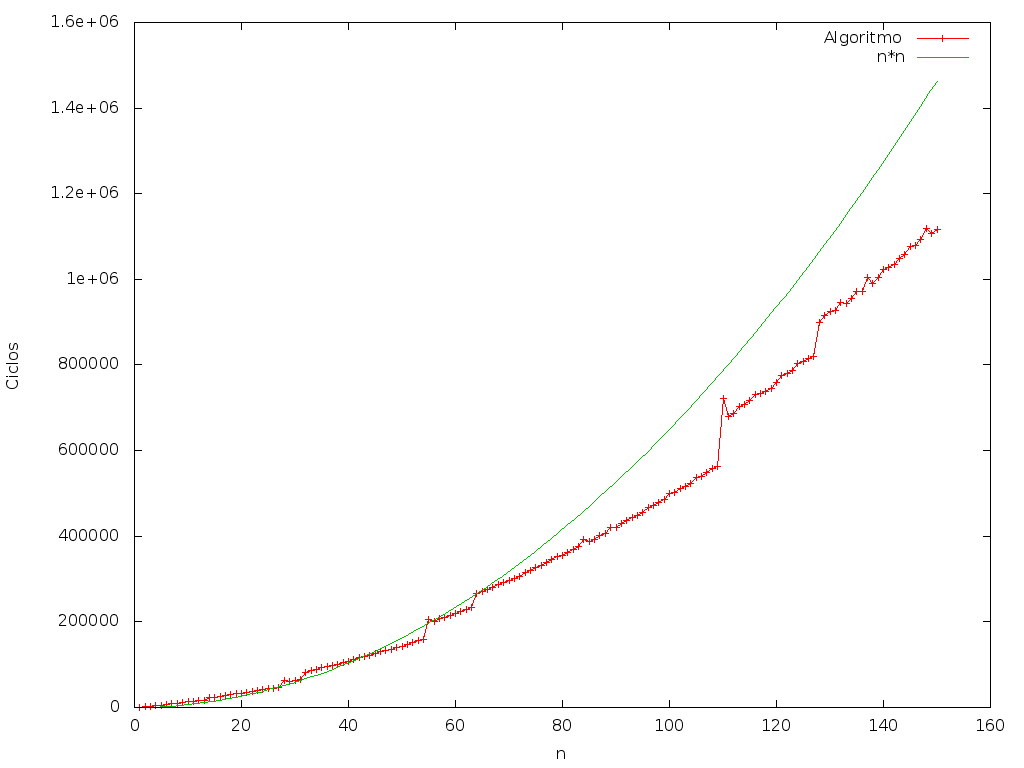
\includegraphics[scale=0.4]{../graficador/graficoAleatoriosEj1.png} 
\end{center}

Dada la naturaleza del algoritmo, no existe un peor caso. Ya que siempre debe llenar una matriz $n^{2}$ y buscar el mínimo dentro de la última columna.\\

Conclusiones:
\begin{itemize}
\item La cota calculada teóricamente era correcta.
\item La técnica de programación dinámica es muy efectiva en ciertos casos.
\end{itemize}
%\input{ej1/codigo_relevante.tex}

\newpage

\section{Ejercicio 2.1}
%\subsection{Descripción}
Se tienen n servidores interconectados mediante m enlaces. Los enlaces tienen un costo en función del tráfico que transmiten y todos los enlaces deben transmitir la misma información. El problema a resolver consiste en seleccionar aquellos enlaces que permitan distribuir la información a los n servidores con costo total mínimo.


Veamos un ejemplo; el siguiente grafo tiene como posible solución el subgrafo en rojo cuyo peso total es 38.

\begin{center}
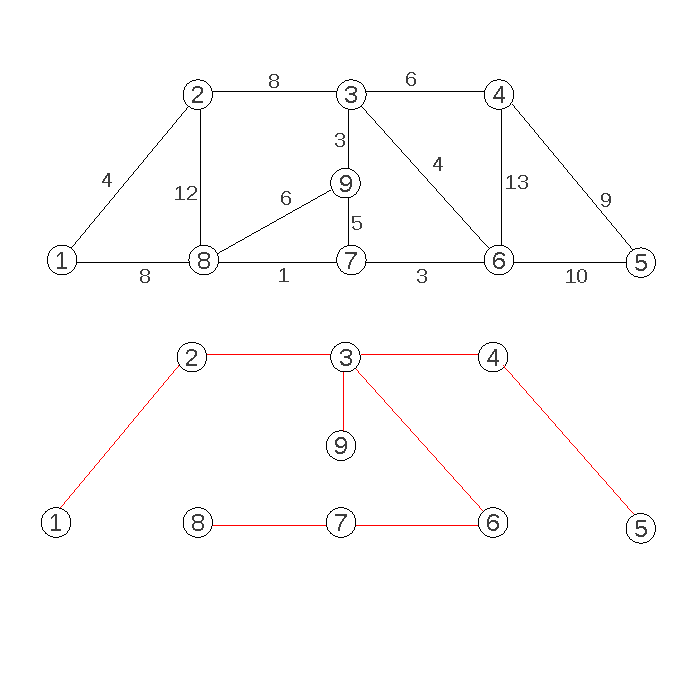
\includegraphics{ej2/1/Img1.pdf} 
\end{center}


%\subsection{Pseudocódigo:}

\begin{algorithm}
\caption{Impresiones ordenadas}\label{ej1}
\begin{algorithmic}[1]
\Procedure{Dividir trabajos}{$n, Costos$}\Comment{n= cant trabajos, Costos= costo de cada trabajo respecto a cada posible anterior}
	\State Inicializo una matriz dp, tamaño n*n
	
	\State dp[0][1]$\gets Costos(1,0)$ \Comment{en la posición (0,1) de la matriz guardo el valor de hacer el trabajo uno primero}
	
	\State $agregar\_a\_maquina2(1)$ \Comment{voy guardando los trabajos para saber al final cómo los dividí}
	
	\For{$j\gets 2, n$} \Comment{el trabajo 1 ya lo agregué}
		\For{$i\gets 0, j-1$}
			\If{$i=j-1$}
				\State $dp[i][j]\gets minimo(dp[i][k]\ +\ Costos(j,\ k),\ \forall\ 0\leq k\leq j-2) $
				\State $agregar\_a\_maquina2(j)$
				
			\Else
				\State $dp[i][j]\gets (dp[i][j-1]\ +\ Costos(j,\ j-1))$
				\State $agregar\_a\_maquina2(j)$
			\EndIf
		\EndFor
	\EndFor
	
	\State \textbf{return} $minimo(dp[i][n], \forall\ 0\leq i\leq n-1)$ 
	\State \Comment{retorno el mínimo de la última columna, además de la combinación para lograr ese mínimo}
\EndProcedure
\end{algorithmic}
\end{algorithm}

\textit{Nota:} Cuando escribo $agregar\_a\_maquina2(j)$ me refiero a agregar j a una lista que depende de la posición de la matriz dp (i.e. hay una para cada posición).\\
%\subsection{Demostración}

Diremos que un conjunto de aristas factible es $prometedor$ si se puede extender para producir no sólo una solución, sino una solución óptima para nuestro problema. Si un conjunto de aristas prometedor ya es solución entonces esta solución debe ser óptima.

La demostración de la correctitud de algoritmo es por inducción sobre el número de aristas que hay en el conjunto T. Demostraremos que si T es prometedor en alguna fase del algoritmo, entonces sigue siendo prometedor al añandir una arista adicional. Cuando se detiene el agoritmo (T tiene C cantidad de aristas), T da una solución prometedora al problema y por lo tanto óptima.

Caso base: el conjunto vacío T es prometedor
Paso inductivo: supongamos que T es prometedor justo antes de que el algoritmo añada una nueva arista $e$ al conjunto T. T es un conjunto de aristas prometedor por hipótesis inductiva y $e$ es por definición una de las aristas más cortas que salen de B. Podemos asegurar que existe un $e$ que cumpla dichos requisitos ya que el enunciado asegura que todos los clientes pueden ser provistos por al menos una fábrica. Por lo tanto T $\cup$ $e$ también es prometedor.

Como el conjunto T es prometedor en todas las fases del algoritmo también lo será cuando finalice ya que ofrece una solción óptima del problema.

%\subsection{Complejidad}

%The running time of Prim’s algorithm depends on how we implement the min-
%priority queue Q. If we implement Q as a binary min-heap (see Chapter 6), we
%can use the B UILD -M IN -H EAP procedure to perform lines 1–5 in O.V / time. The
%body of the while loop executes jV j times, and since each E XTRACT-M IN opera-
%tion takes O.lg V / time, the total time for all calls to E XTRACT-M IN is O.V lg V /.
%The for loop in lines 8–11 executes O.E/ times altogether, since the sum of the
%lengths of all adjacency lists is 2 jEj. Within the for loop, we can implement the
%test for membership in Q in line 9 in constant time by keeping a bit for each vertex
%that tells whether or not it is in Q, and updating the bit when the vertex is removed
%5from Q. The assignment in line 11 involves an implicit D ECREASE -K EY opera-
%tion on the min-heap, which a binary min-heap supports in O.lg V / time. Thus,
%the total time for Prim’s algorithm is O.V lg V C E lg V / D O.E lg V /, which is
%asymptotically the same as for our implementation of Kruskal’s algorithm.

La complejidad de Prim Modificado dependerá de la estructura utilizada para ir eligiendo aristas. El cuerpo del while se ejecuta C veces. El obtener mínimo dentro del while se ejecutará O(R) veces en total en donde cada operación de push, pop cuesta log(R) lo que equivale a O(log $(F+C)^2$) ya que $(F+C)^2$ es la mayor cantidad de aristas posibles. Como F es menor que C (enunciado), log($(C+F)^2$) $\subset$ log($C^2$). Por lo tanto la complejidad equivale a O(2 log C) $\subset$ O(log C). El for que se encarga de pushear las aristas adyacentes a la cola de prioridad también se ejecutará un total de R veces y la operación de push cuesta log(R) $\subset$ O(log C). Por lo tanto la complejidad total será de O(R*log(C)+R*log(C)) $\subset$ O(R*log(C)) como pedía el enunciado.

%\input{ej2/1/codigo_relevante.tex}
%\newpage

\section{Ejercicio 2.2}
\subsection{Descripción}
Se tienen n servidores interconectados mediante m enlaces. Los enlaces tienen un costo en función del tráfico que transmiten y todos los enlaces deben transmitir la misma información. El problema a resolver consiste en seleccionar aquellos enlaces que permitan distribuir la información a los n servidores con costo total mínimo.


Veamos un ejemplo; el siguiente grafo tiene como posible solución el subgrafo en rojo cuyo peso total es 38.

\begin{center}
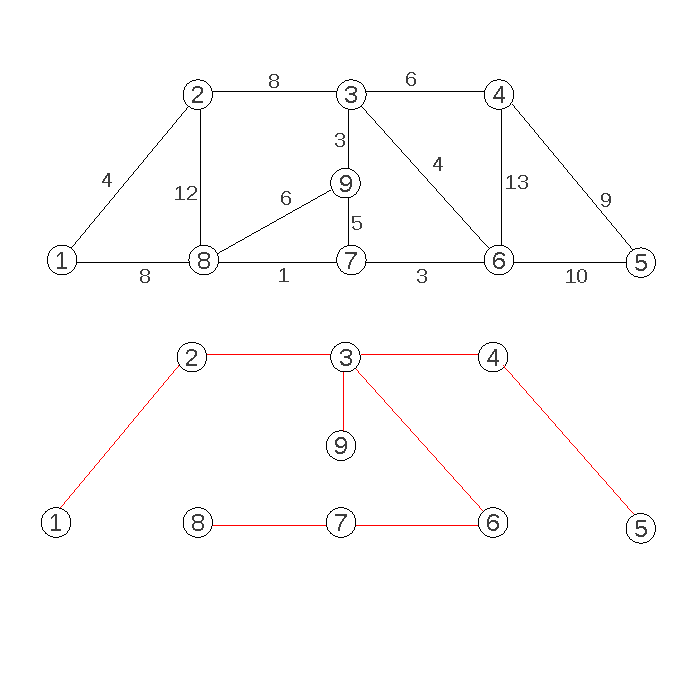
\includegraphics{ej2/1/Img1.pdf} 
\end{center}


\subsection{Pseudocódigo:}

\begin{algorithm}
\caption{Impresiones ordenadas}\label{ej1}
\begin{algorithmic}[1]
\Procedure{Dividir trabajos}{$n, Costos$}\Comment{n= cant trabajos, Costos= costo de cada trabajo respecto a cada posible anterior}
	\State Inicializo una matriz dp, tamaño n*n
	
	\State dp[0][1]$\gets Costos(1,0)$ \Comment{en la posición (0,1) de la matriz guardo el valor de hacer el trabajo uno primero}
	
	\State $agregar\_a\_maquina2(1)$ \Comment{voy guardando los trabajos para saber al final cómo los dividí}
	
	\For{$j\gets 2, n$} \Comment{el trabajo 1 ya lo agregué}
		\For{$i\gets 0, j-1$}
			\If{$i=j-1$}
				\State $dp[i][j]\gets minimo(dp[i][k]\ +\ Costos(j,\ k),\ \forall\ 0\leq k\leq j-2) $
				\State $agregar\_a\_maquina2(j)$
				
			\Else
				\State $dp[i][j]\gets (dp[i][j-1]\ +\ Costos(j,\ j-1))$
				\State $agregar\_a\_maquina2(j)$
			\EndIf
		\EndFor
	\EndFor
	
	\State \textbf{return} $minimo(dp[i][n], \forall\ 0\leq i\leq n-1)$ 
	\State \Comment{retorno el mínimo de la última columna, además de la combinación para lograr ese mínimo}
\EndProcedure
\end{algorithmic}
\end{algorithm}

\textit{Nota:} Cuando escribo $agregar\_a\_maquina2(j)$ me refiero a agregar j a una lista que depende de la posición de la matriz dp (i.e. hay una para cada posición).\\
\subsection{Complejidad}

%The running time of Prim’s algorithm depends on how we implement the min-
%priority queue Q. If we implement Q as a binary min-heap (see Chapter 6), we
%can use the B UILD -M IN -H EAP procedure to perform lines 1–5 in O.V / time. The
%body of the while loop executes jV j times, and since each E XTRACT-M IN opera-
%tion takes O.lg V / time, the total time for all calls to E XTRACT-M IN is O.V lg V /.
%The for loop in lines 8–11 executes O.E/ times altogether, since the sum of the
%lengths of all adjacency lists is 2 jEj. Within the for loop, we can implement the
%test for membership in Q in line 9 in constant time by keeping a bit for each vertex
%that tells whether or not it is in Q, and updating the bit when the vertex is removed
%5from Q. The assignment in line 11 involves an implicit D ECREASE -K EY opera-
%tion on the min-heap, which a binary min-heap supports in O.lg V / time. Thus,
%the total time for Prim’s algorithm is O.V lg V C E lg V / D O.E lg V /, which is
%asymptotically the same as for our implementation of Kruskal’s algorithm.

La complejidad de Prim Modificado dependerá de la estructura utilizada para ir eligiendo aristas. El cuerpo del while se ejecuta C veces. El obtener mínimo dentro del while se ejecutará O(R) veces en total en donde cada operación de push, pop cuesta log(R) lo que equivale a O(log $(F+C)^2$) ya que $(F+C)^2$ es la mayor cantidad de aristas posibles. Como F es menor que C (enunciado), log($(C+F)^2$) $\subset$ log($C^2$). Por lo tanto la complejidad equivale a O(2 log C) $\subset$ O(log C). El for que se encarga de pushear las aristas adyacentes a la cola de prioridad también se ejecutará un total de R veces y la operación de push cuesta log(R) $\subset$ O(log C). Por lo tanto la complejidad total será de O(R*log(C)+R*log(C)) $\subset$ O(R*log(C)) como pedía el enunciado.

\subsection{Demostración}

Diremos que un conjunto de aristas factible es $prometedor$ si se puede extender para producir no sólo una solución, sino una solución óptima para nuestro problema. Si un conjunto de aristas prometedor ya es solución entonces esta solución debe ser óptima.

La demostración de la correctitud de algoritmo es por inducción sobre el número de aristas que hay en el conjunto T. Demostraremos que si T es prometedor en alguna fase del algoritmo, entonces sigue siendo prometedor al añandir una arista adicional. Cuando se detiene el agoritmo (T tiene C cantidad de aristas), T da una solución prometedora al problema y por lo tanto óptima.

Caso base: el conjunto vacío T es prometedor
Paso inductivo: supongamos que T es prometedor justo antes de que el algoritmo añada una nueva arista $e$ al conjunto T. T es un conjunto de aristas prometedor por hipótesis inductiva y $e$ es por definición una de las aristas más cortas que salen de B. Podemos asegurar que existe un $e$ que cumpla dichos requisitos ya que el enunciado asegura que todos los clientes pueden ser provistos por al menos una fábrica. Por lo tanto T $\cup$ $e$ también es prometedor.

Como el conjunto T es prometedor en todas las fases del algoritmo también lo será cuando finalice ya que ofrece una solción óptima del problema.

\subsection{Casos de Prueba}

Vamos a presentar 5 instancias distintas del problema mediante gr´aficos, y la soluci´on que nos devuelve la implementaci´on, de manera de hacer una comprobaci´on visual del funcionamiento.

\begin{center}
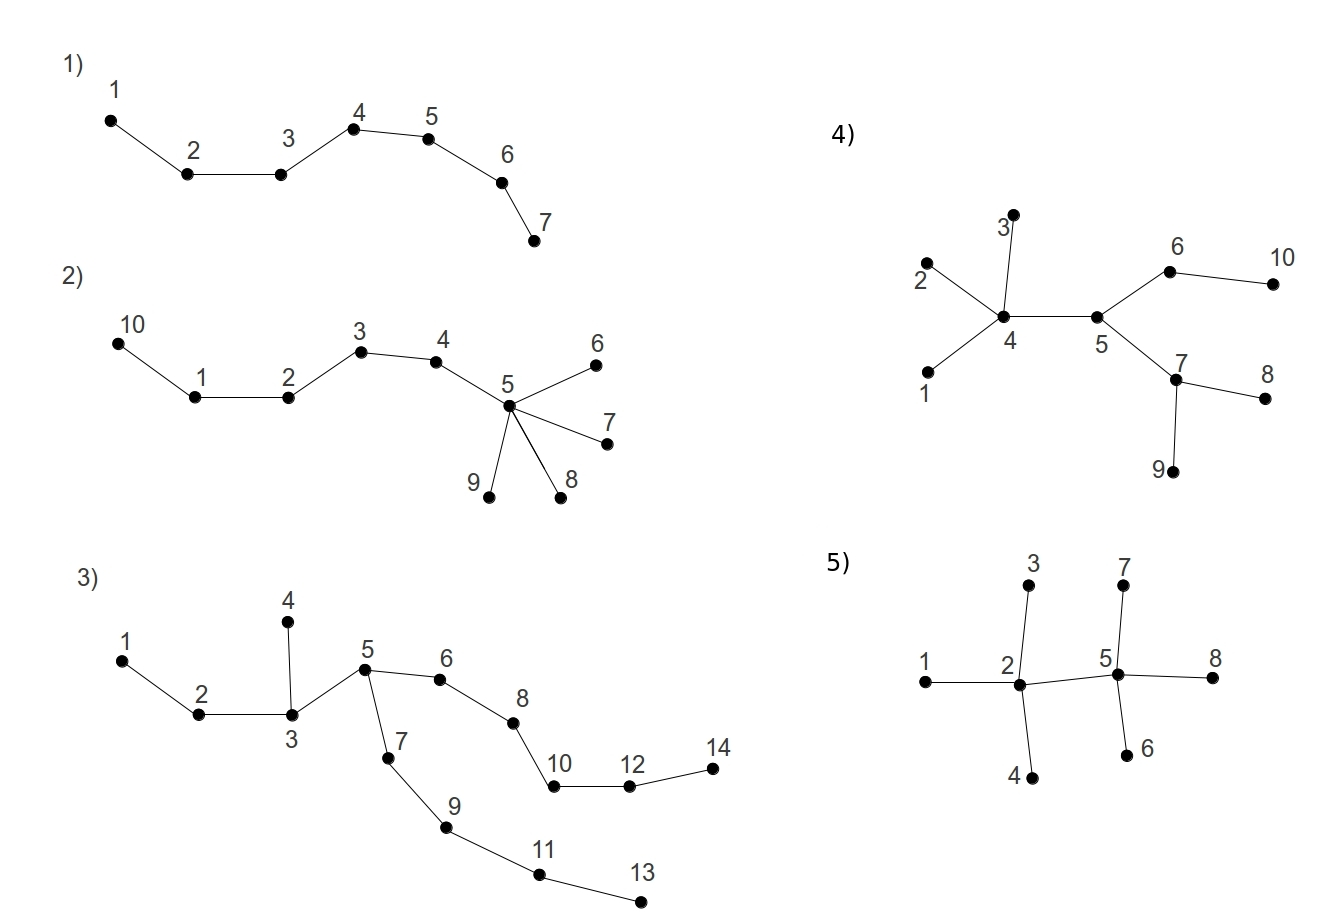
\includegraphics[scale=0.5]{ej2/2/graficos/imagen05.jpg} 
\end{center}

\begin{center}
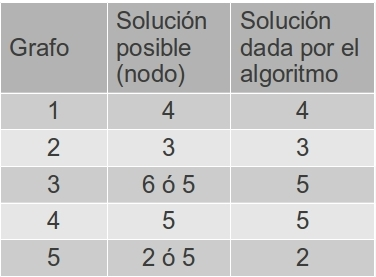
\includegraphics[scale=0.5]{ej2/2/graficos/imagen06.jpg} 
\end{center}
\subsection{Preguntas Adicionales}
Es posible resolver las dos partes por separado de forma óptima y que aún así haya una solución en la que la replicación termine en menos tiempo, como muestra el ejemplo a continuación.
\begin{center}
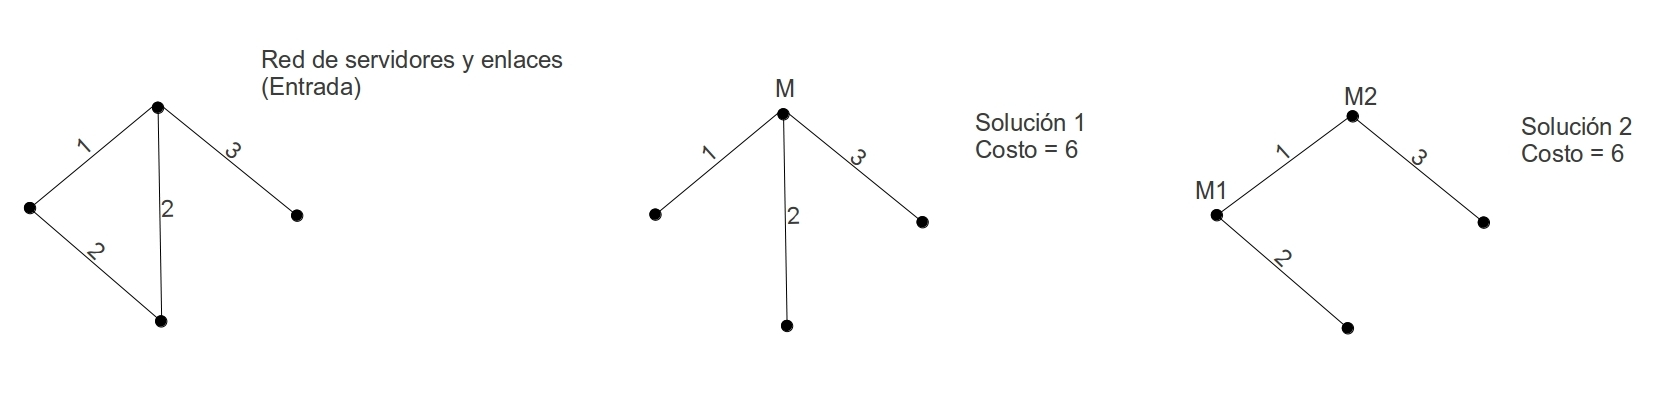
\includegraphics[scale=0.4]{ej2/2/graficos/imagen07.jpg} 
\end{center}
Tenemos dos soluciones posibles para el primer problema,
%\input{ej2/2/codigo_relevante.tex}
%\subsection{Experimentación}

Para medir empiricamente la eficiencia del algoritmo decidimos tomar varias instancias del problema con grafos G cuya cantidad de nodos (n) va desde 5 a 200. Los grafos generados tendrán n/2-1 fábricas y n-n/2-1 clientes de manera que se cumple que la cantidad de fábricas sea menor a la de clientes. Además, la cantidad de aristas será (n(n-1))/2 lo cual nos forma grafos completos. Graficamos los resultados de los ciclos insumidos en función del número de aristas presentes en el grafo. Los resultados obtenidos fueron los siguientes:

\begin{figure}[H]
\center
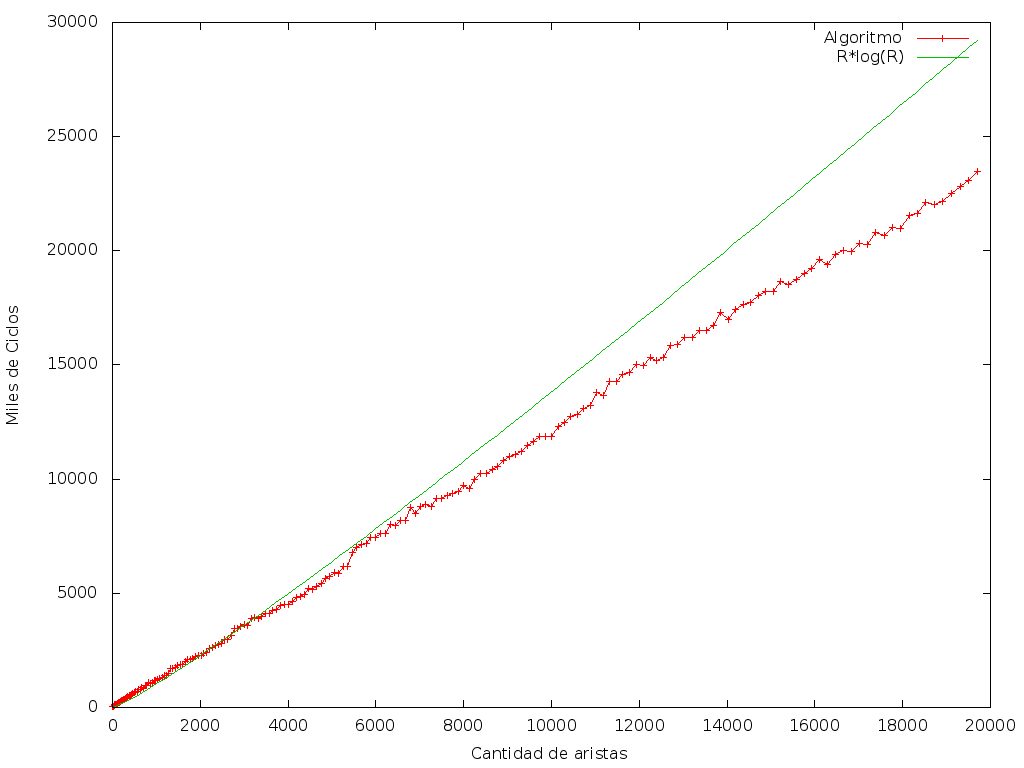
\includegraphics[scale=0.40]{ej3/imgs/complejidad.png}
\caption[Long caption]{Gráfico de complejidad para grafos completos que van desde 5 a 200 nodos.}
\label{pic-a}
\end{figure}

Como fue mencionado en la sección 4.3 (Implementación y complejidad), O(log(R))=O(log($(C+F)^2$))$\subset$ log($C^2$)=O(2 log C)$\subset$ O(log C) por lo cual mostrar que se encuentra acotado por Rlog(R) es equivalente a hacerlo por Rlog(C). Como el gráfico es de dos dimensiones, no podemos incluir la variable C al gráfico por lo cual sólo graficamos en función de la cantidad de aristas.

Viendo el gráfico podemos apreciar que el algoritmo se encuentra acotado por O(Rlog(R)) como pedía el enunciado.



\newpage

\section{Ejercicio 3}
\subsection{Descripción}
Se tienen n servidores interconectados mediante m enlaces. Los enlaces tienen un costo en función del tráfico que transmiten y todos los enlaces deben transmitir la misma información. El problema a resolver consiste en seleccionar aquellos enlaces que permitan distribuir la información a los n servidores con costo total mínimo.


Veamos un ejemplo; el siguiente grafo tiene como posible solución el subgrafo en rojo cuyo peso total es 38.

\begin{center}
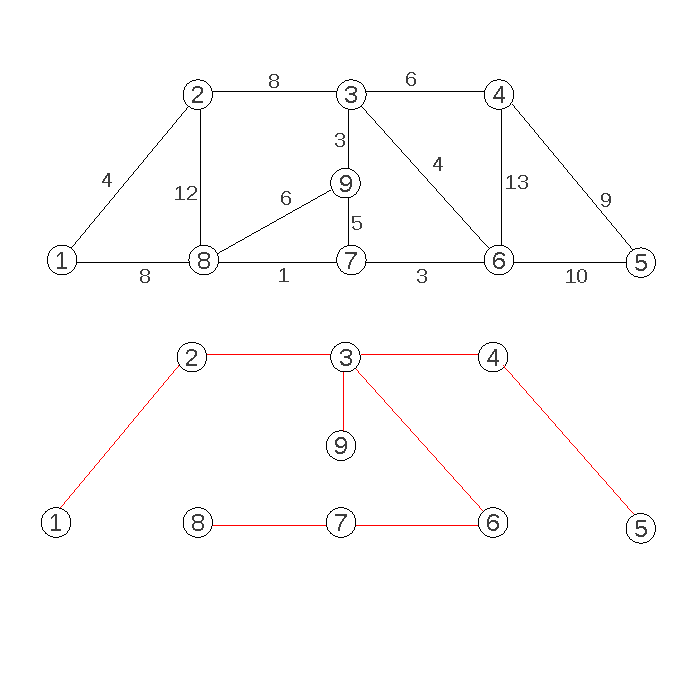
\includegraphics{ej2/1/Img1.pdf} 
\end{center}


\subsection{Pseudocódigo:}

\begin{algorithm}
\caption{Impresiones ordenadas}\label{ej1}
\begin{algorithmic}[1]
\Procedure{Dividir trabajos}{$n, Costos$}\Comment{n= cant trabajos, Costos= costo de cada trabajo respecto a cada posible anterior}
	\State Inicializo una matriz dp, tamaño n*n
	
	\State dp[0][1]$\gets Costos(1,0)$ \Comment{en la posición (0,1) de la matriz guardo el valor de hacer el trabajo uno primero}
	
	\State $agregar\_a\_maquina2(1)$ \Comment{voy guardando los trabajos para saber al final cómo los dividí}
	
	\For{$j\gets 2, n$} \Comment{el trabajo 1 ya lo agregué}
		\For{$i\gets 0, j-1$}
			\If{$i=j-1$}
				\State $dp[i][j]\gets minimo(dp[i][k]\ +\ Costos(j,\ k),\ \forall\ 0\leq k\leq j-2) $
				\State $agregar\_a\_maquina2(j)$
				
			\Else
				\State $dp[i][j]\gets (dp[i][j-1]\ +\ Costos(j,\ j-1))$
				\State $agregar\_a\_maquina2(j)$
			\EndIf
		\EndFor
	\EndFor
	
	\State \textbf{return} $minimo(dp[i][n], \forall\ 0\leq i\leq n-1)$ 
	\State \Comment{retorno el mínimo de la última columna, además de la combinación para lograr ese mínimo}
\EndProcedure
\end{algorithmic}
\end{algorithm}

\textit{Nota:} Cuando escribo $agregar\_a\_maquina2(j)$ me refiero a agregar j a una lista que depende de la posición de la matriz dp (i.e. hay una para cada posición).\\
\subsection{Complejidad}

%The running time of Prim’s algorithm depends on how we implement the min-
%priority queue Q. If we implement Q as a binary min-heap (see Chapter 6), we
%can use the B UILD -M IN -H EAP procedure to perform lines 1–5 in O.V / time. The
%body of the while loop executes jV j times, and since each E XTRACT-M IN opera-
%tion takes O.lg V / time, the total time for all calls to E XTRACT-M IN is O.V lg V /.
%The for loop in lines 8–11 executes O.E/ times altogether, since the sum of the
%lengths of all adjacency lists is 2 jEj. Within the for loop, we can implement the
%test for membership in Q in line 9 in constant time by keeping a bit for each vertex
%that tells whether or not it is in Q, and updating the bit when the vertex is removed
%5from Q. The assignment in line 11 involves an implicit D ECREASE -K EY opera-
%tion on the min-heap, which a binary min-heap supports in O.lg V / time. Thus,
%the total time for Prim’s algorithm is O.V lg V C E lg V / D O.E lg V /, which is
%asymptotically the same as for our implementation of Kruskal’s algorithm.

La complejidad de Prim Modificado dependerá de la estructura utilizada para ir eligiendo aristas. El cuerpo del while se ejecuta C veces. El obtener mínimo dentro del while se ejecutará O(R) veces en total en donde cada operación de push, pop cuesta log(R) lo que equivale a O(log $(F+C)^2$) ya que $(F+C)^2$ es la mayor cantidad de aristas posibles. Como F es menor que C (enunciado), log($(C+F)^2$) $\subset$ log($C^2$). Por lo tanto la complejidad equivale a O(2 log C) $\subset$ O(log C). El for que se encarga de pushear las aristas adyacentes a la cola de prioridad también se ejecutará un total de R veces y la operación de push cuesta log(R) $\subset$ O(log C). Por lo tanto la complejidad total será de O(R*log(C)+R*log(C)) $\subset$ O(R*log(C)) como pedía el enunciado.

\subsection{Demostración}

Diremos que un conjunto de aristas factible es $prometedor$ si se puede extender para producir no sólo una solución, sino una solución óptima para nuestro problema. Si un conjunto de aristas prometedor ya es solución entonces esta solución debe ser óptima.

La demostración de la correctitud de algoritmo es por inducción sobre el número de aristas que hay en el conjunto T. Demostraremos que si T es prometedor en alguna fase del algoritmo, entonces sigue siendo prometedor al añandir una arista adicional. Cuando se detiene el agoritmo (T tiene C cantidad de aristas), T da una solución prometedora al problema y por lo tanto óptima.

Caso base: el conjunto vacío T es prometedor
Paso inductivo: supongamos que T es prometedor justo antes de que el algoritmo añada una nueva arista $e$ al conjunto T. T es un conjunto de aristas prometedor por hipótesis inductiva y $e$ es por definición una de las aristas más cortas que salen de B. Podemos asegurar que existe un $e$ que cumpla dichos requisitos ya que el enunciado asegura que todos los clientes pueden ser provistos por al menos una fábrica. Por lo tanto T $\cup$ $e$ también es prometedor.

Como el conjunto T es prometedor en todas las fases del algoritmo también lo será cuando finalice ya que ofrece una solción óptima del problema.

\subsection{Casos de Prueba}

Vamos a presentar 5 instancias distintas del problema mediante gr´aficos, y la soluci´on que nos devuelve la implementaci´on, de manera de hacer una comprobaci´on visual del funcionamiento.

\begin{center}
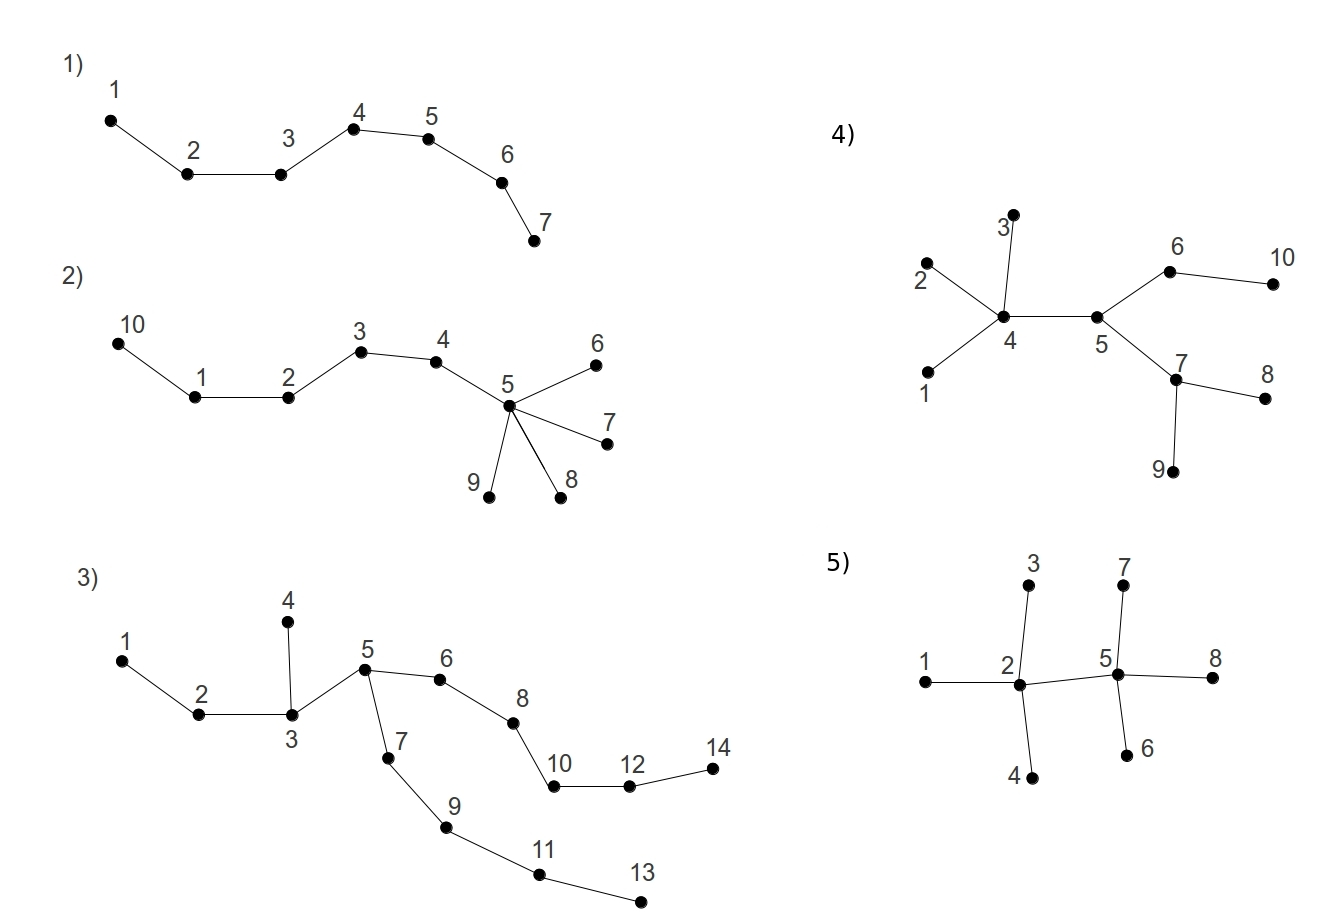
\includegraphics[scale=0.5]{ej2/2/graficos/imagen05.jpg} 
\end{center}

\begin{center}
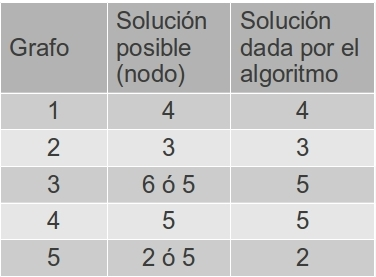
\includegraphics[scale=0.5]{ej2/2/graficos/imagen06.jpg} 
\end{center}
%\input{ej3/codigo_relevante.tex}
\subsection{Experimentación}

Para medir empiricamente la eficiencia del algoritmo decidimos tomar varias instancias del problema con grafos G cuya cantidad de nodos (n) va desde 5 a 200. Los grafos generados tendrán n/2-1 fábricas y n-n/2-1 clientes de manera que se cumple que la cantidad de fábricas sea menor a la de clientes. Además, la cantidad de aristas será (n(n-1))/2 lo cual nos forma grafos completos. Graficamos los resultados de los ciclos insumidos en función del número de aristas presentes en el grafo. Los resultados obtenidos fueron los siguientes:

\begin{figure}[H]
\center
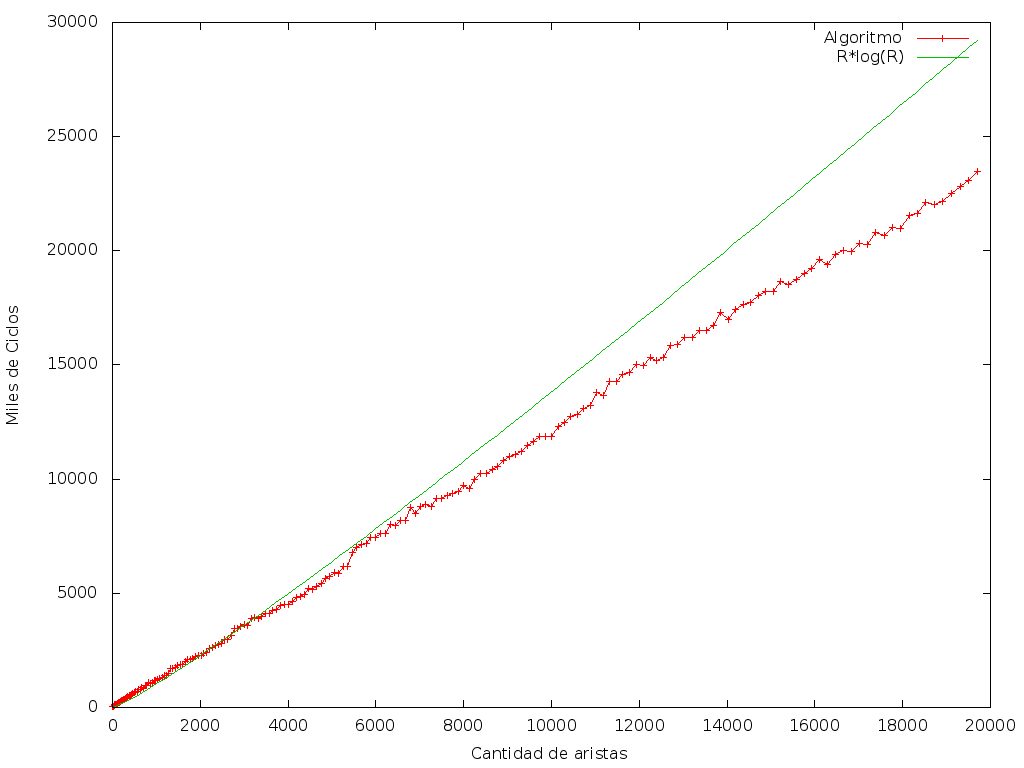
\includegraphics[scale=0.40]{ej3/imgs/complejidad.png}
\caption[Long caption]{Gráfico de complejidad para grafos completos que van desde 5 a 200 nodos.}
\label{pic-a}
\end{figure}

Como fue mencionado en la sección 4.3 (Implementación y complejidad), O(log(R))=O(log($(C+F)^2$))$\subset$ log($C^2$)=O(2 log C)$\subset$ O(log C) por lo cual mostrar que se encuentra acotado por Rlog(R) es equivalente a hacerlo por Rlog(C). Como el gráfico es de dos dimensiones, no podemos incluir la variable C al gráfico por lo cual sólo graficamos en función de la cantidad de aristas.

Viendo el gráfico podemos apreciar que el algoritmo se encuentra acotado por O(Rlog(R)) como pedía el enunciado.



\end{document}
